\documentclass[12pt]{article}
\usepackage[top = 2.5cm, bottom = 2.5cm, right = 2.5cm, left = 2.5cm]{geometry}
\usepackage{graphicx,float}
\usepackage{tikz}
\usetikzlibrary{shapes,snakes,arrows,chains}
\usetikzlibrary[calc]
\usepackage{amsmath}
\usepackage[pdftex,pdfauthor={Pavithran S Iyer}, pdftitle={Converting between channel representations}]{hyperref}
\hypersetup{
    colorlinks,
    citecolor=blue,
    filecolor=blue,
    linkcolor=blue,
    urlcolor=blue
}
%%%%%%%%%%
% Macros
\def\cE{\mathcal{E}}
\def\tr{\mathsf{Tr}}
%%%%%%%%%%

\begin{document}
\section{Converting between channel representations}

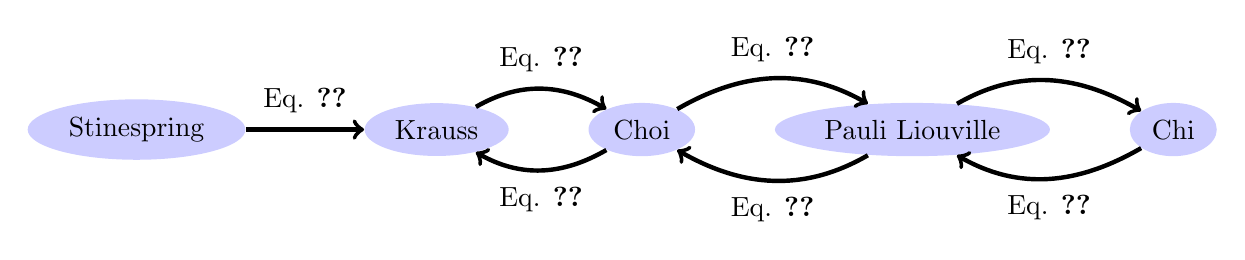
\begin{tikzpicture}[node distance=1cm,auto]
\node[ellipse, fill=blue!20] (p1) {Choi};
\node[ellipse, left=1cm of p1, fill=blue!20] (p2) {Krauss};
\node[ellipse, left=1.5cm of p2, fill=blue!20] (p3) {Stinespring};
\node[ellipse, right=1cm of p1, fill=blue!20] (p4) {Pauli Liouville};
\node[ellipse, right=1cm of p4, fill=blue!20] (p5) {Chi};
\path[draw,ultra thick,->] (p1) to[out=210,in=-30] node[below=0.2em]{Eq. \ref{choi_krauss}} (p2);
\path[draw,ultra thick,->] (p2) to[out=30,in=150] node[above=0.2em]{Eq. \ref{krauss_choi}} (p1);
\path[draw,ultra thick,->] (p3) to[out=0,in=180] node[above=0.2em]{Eq. \ref{stine_krauss}} (p2);
\path[draw,ultra thick,->] (p1) to[out=30,in=150] node[above=0.2em]{Eq. \ref{choi_process}} (p4);
\path[draw,ultra thick,->] (p4) to[out=210,in=-30] node[below=0.2em]{Eq. \ref{process_choi}} (p1);
\path[draw,ultra thick,->] (p4) to[out=30,in=150] node[above=0.2em]{Eq. \ref{process_chi}} (p5);
\path[draw,ultra thick,->] (p5) to[out=210,in=-30] node[below=0.2em]{Eq. \ref{chi_process}} (p4);
\end{tikzpicture}


\begin{enumerate}
\item Krauss operators $\rightarrow$ Pauli Liouville matrix.

Input: $\{K_{i}\}_{k=1}^{r}$, where each of $K_{i}$ are $2 \times 2$ matrices.
Output: $\Gamma$, a $4 \times 4$ real matrix.

The entries of $\Gamma$ are given by the following expression.
\begin{gather}
\Gamma_{i,j} = \tr(\cE(P_{i})P_{j}) \label{process}
\end{gather}
where $\cE$ is the CPTP map described by the input Krauss operators, as in (Eq. \ref{krauss}) and $P_{i}$ is one of the Pauli matrices $\{I, X, Y, Z\}$. So, the process matrix can be expressed in terms of the Krauss operators as
\begin{gather}
\Gamma_{i,j} = \sum_{k = 1}^{r}\tr(K_{k}P_{i}K^{\dagger}_{k}P_{j}) . \label{krauss_process}
\end{gather}

\item Krauss operators $\rightarrow$ Choi Matrix

Input: $\{K_{i}\}_{k=1}^{r}$, where each of $K_{i}$ are $2 \times 2$ matrices.
Output: $J$, a $4 \times 4$ complex matrix.

The Choi matrix of a CPTP map $\cE$ (specified by the input Krauss operators) is the result of applying $\cE$ on the first qubit of a bell state, i.e,
\begin{flalign}
J &= \dfrac{1}{4}\sum_{i,j = 0}^{1}\cE(|i\rangle\langle j|) \otimes |i\rangle\langle j| \label{choi} \\
&= \dfrac{1}{4}\sum_{i,j = 0}^{1}\sum_{k = 1}^{r}K_{k}|i\rangle\langle j|K^{\dagger}_{k} \otimes |i\rangle\langle j| \label{krauss_choi}
\end{flalign}

\item $\chi$ matrix $\rightarrow$ Pauli Liouville Matrix

Input: $\chi$, a $4 \times 4$ complex matrix.
Output: $\Gamma$, a $4 \times 4$ real matrix.

The action of a CPTP map $\cE$ on an input state $\rho$ is specified using its $\chi$ matrix as
\begin{gather}
\cE(\rho) = \sum_{l,m}\chi_{l,m}P_{l}\rho P_{m} \label{chi}.
\end{gather}
Using the definition of the process matrix $\Gamma$, corresponding to the CPTP map $\cE$, in (Eq. \ref{process}), we have
\begin{gather*}
\Gamma_{i,j} = \sum_{l,m}\tr(P_{l} P_{i} P_{m} P_{j})\chi_{l,m} .
\end{gather*}
Defining a $16\times 16$ matrix $\Omega$, such that $\Omega_{4 \times i + j, 4 \times l + m} = \tr(P_{l} P_{i} P_{m} P_{j})$, we have
\begin{gather}
|\Gamma\rangle\rangle = \Omega|\chi\rangle\rangle \label{chi_process} ,
\end{gather}
where $|\Gamma\rangle\rangle$ and $|\chi\rangle\rangle$ are the (column) vectorized forms of $\Gamma$ and $\chi$ respectively.

\item Pauli Liouville Matrix $\rightarrow$ $\chi$ matrix.

We can easily obtain $|\chi\rangle\rangle$ by inverting the relation in Eq. \ref{chi_process}, giving
\begin{gather}
|\chi\rangle\rangle = \Omega^{-1}|\Gamma\rangle\rangle \label{process_chi} .
\end{gather}

\item Choi Matrix $\rightarrow$ Krauss operators.

Input: $J$, a $4 \times 4$ complex matrix.
Output: $\{K_{i}\}_{k=1}^{r}$, where each of $K_{i}$ are $2 \times 2$ matrices.

Eq. \ref{krauss_choi} can be expressed as
\begin{gather}
J = \sum_{k = 1}^{r}|K_{k}\rangle\rangle\langle\langle K_{k}| \label{choi_krauss},
\end{gather}
where $|K_{k}\rangle\rangle$ is the (column) vectorized form of the Krauss operator $\dfrac{1}{2}K_{k}$. Performing a singular value decomposition of $J$, we find $J = \sum_{k}\lambda_{k}|\lambda_{k}\rangle\langle\lambda_{k}|$. Hence the Krauss operator $K_{k}$ can be constructed from un-vectorizing $2|\lambda_{k}\rangle$.

\item Pauli Liouville Matrix $\rightarrow$ Choi Matrix

Input: $\Gamma$, a $4 \times 4$ real matrix.
Output: $J$, a $4 \times 4$ complex matrix.

Combining the expression for the bell state in the Pauli basis,
\begin{gather*}
\dfrac{1}{4}(|00\rangle + |11\rangle)(\langle00| + \langle11|) = \dfrac{1}{4}\sum_{i = 1}^{4}P_{i} \otimes P^{T}_{i},
\end{gather*}
where $P_{i} \in \{I, X, Y, Z\}$ is a Pauli matrix, with Eq. \ref{choi}, we find
\begin{gather*}
J = \dfrac{1}{4}\sum_{i}\cE(P_{i})\otimes P^{T}_{i} .
\end{gather*}
Applying the definition of the Pauli Liouville representation of $\cE$ in Eq. \ref{process}, we find
\begin{gather}
J = \sum_{i,j}\Gamma_{i,j}P_{j} \otimes P^{T}_{i} \label{process_choi} .
\end{gather}

\item Choi Matrix $\rightarrow$ Pauli Liouville Matrix.

Input: $J$, a $4 \times 4$ complex matrix.
Output: $\Gamma$, a $4 \times 4$ real matrix.

Multiplying on either sides of Eq. \ref{process_choi} by $P_{a}\otimes P^{T}_{b}$, we find
\begin{gather}
J \cdot (P_{a} \otimes P^{T}_{b}) = \sum_{i,j} \Gamma_{i,j} P_{j}P_{a} \otimes P^{T}_{i}P^{T}_{b} \nonumber .
\end{gather}
Taking the trace of the above equation yields
\begin{gather}
\Gamma_{b,a} = \tr(J \cdot (P_{a}\otimes P^{T}_{b})) \label{choi_process} .
\end{gather}

\item Strinespring dilation $\rightarrow$ Krauss operators.

The action of any CPTP map $\cE$ on an input state $\rho$ can be derived from unitary dynamics $U$ on a larger Hilbert space, that comprises of the system $\rho$ and its environment, which is initially in some state $|0\rangle_{E}\langle0|_{E}$. Under the unitary evolution described by $U$, we find
\begin{gather*}
\rho \otimes |0\rangle_{E}\langle0|_{E} \rightarrow U \left[\rho \otimes |0\rangle_{E}\langle0|_{E}\right] U^{\dagger} .
\end{gather*}
Since the state of the environment is essentially unknown, we must discard it resulting in a partial trace over the environment basis, denoted by $\{|e_{k}\rangle_{E}\}$, resulting in
\begin{flalign}
\rho \otimes |0\rangle_{E}\langle0|_{E} \rightarrow& \tr_{E}\left(U \left[\rho \otimes |0\rangle_{E}\langle0|_{E}\right] U^{\dagger}\right) \nonumber \\
=& \rho_{ab}\sum_{k=1}^{r}\langle e_{k}|U|e_{0}\rangle \rho \langle e_{0}|U^{\dagger}|e_{k}\rangle \label{stine_krauss}.
\end{flalign}
The above expression is the Krauss representation of the channel where the Krauss operators are $\{\langle e_{k}|U|e_{0}\rangle\}_{k=1}^{r}$.
\end{enumerate}

\begin{figure}[H]
\begin{center}
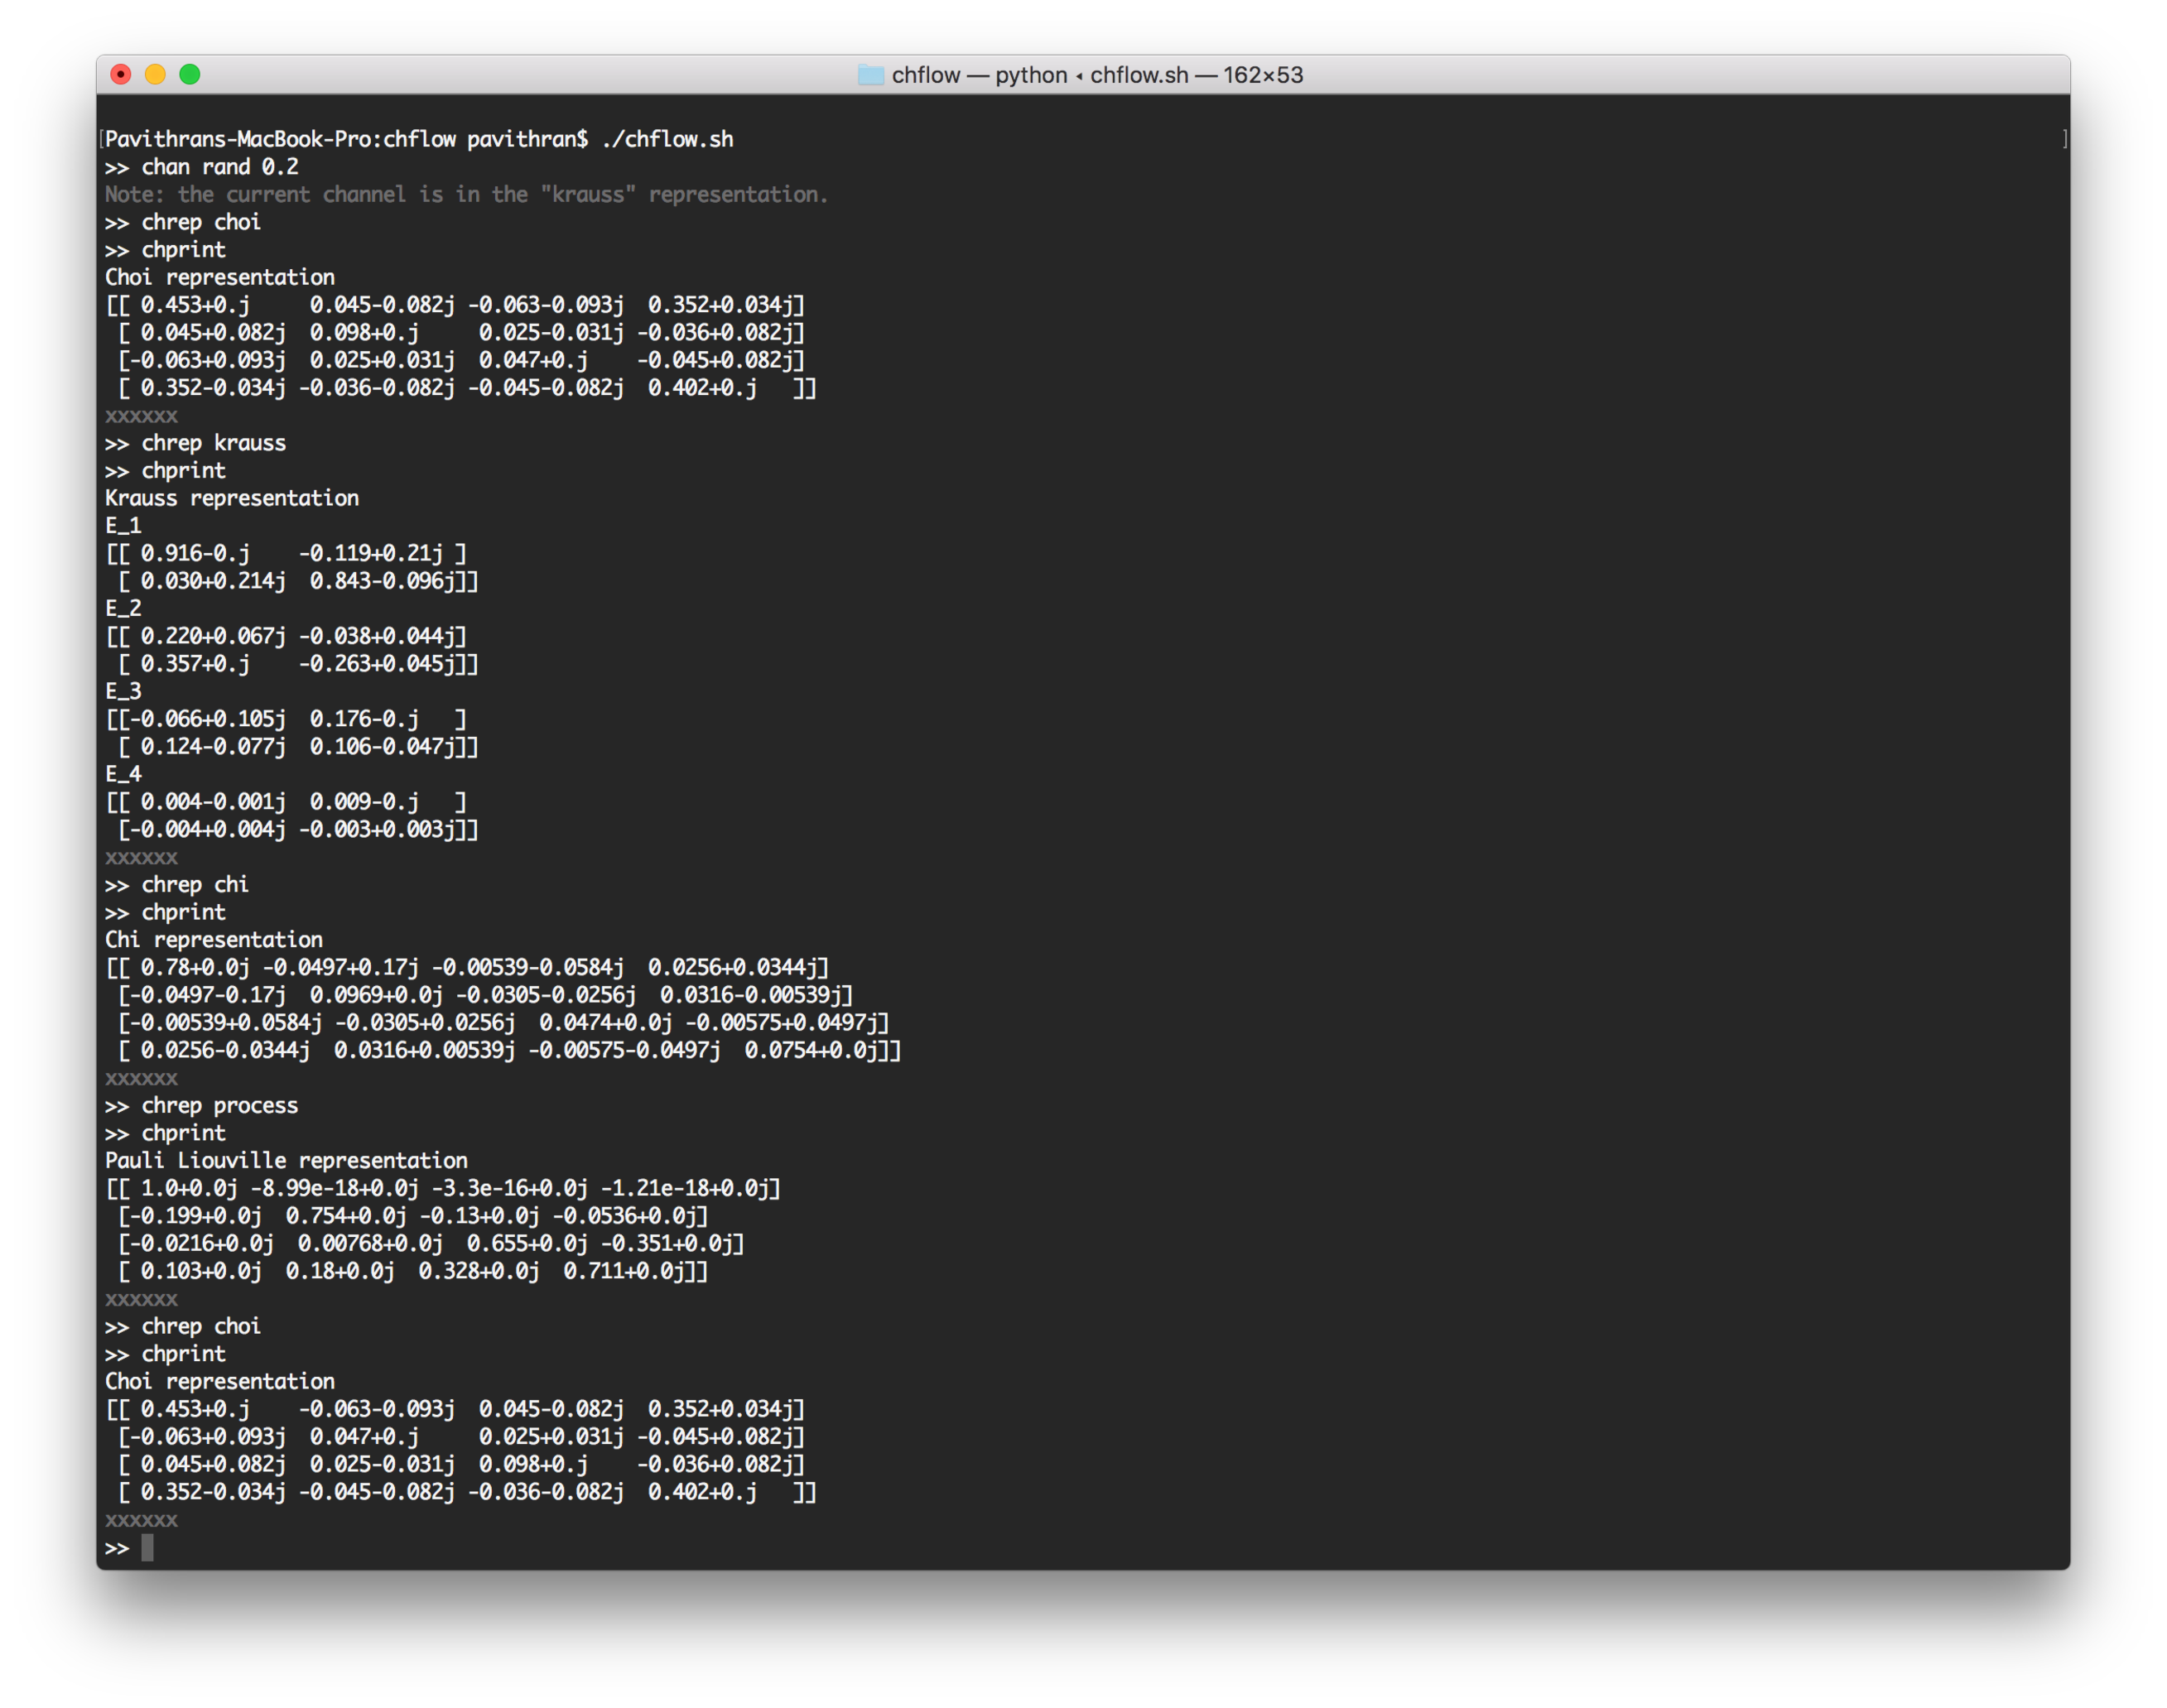
\includegraphics[scale=0.4]{chreps_screen.pdf}
\caption{The \texttt{chrep} command in chflow can be used to change channel representations. The usage of the command is \texttt{chrep <representation>}, where \texttt{<representation>} should be replaced by one of \{\texttt{krauss}, \texttt{process}, \texttt{choi}, \texttt{chi}, \texttt{stine}\}, which results in the current channel being stored in the specified representation.}
\label{fig:chrep_screen}
\end{center}
\end{figure}

\end{document}